\documentclass[aspectratio=169,14pt,usenames,dvipsnames]{beamer}

\usepackage[utf8]{inputenc}
\usepackage{fontspec}
\usepackage{enumitem}
\usepackage{calc}

\usepackage{datetime}
\newcommand\builddate{%
   \ifcase \month%
        \or Janeiro%
        \or Fevereiro%
        \or Março%
        \or Abril%
        \or Maio%
        \or Junho%
        \or Julho%
        \or Agosto%
        \or Setembro%
        \or Outubro%
        \or Novembro%
        \or Dezembro%
    \fi\space\number\year%
}

\newcommand{\loadtheme}[1]{%
    \input{themes/#1}%
}
\newcommand{\presentationlanguage}[1]{%
    \usepackage[#1]{babel}%
}

\newcommand{\usecodingsamples}[1]{%
    \usepackage{listings}%
    \input{listings/#1}%
}

% Configura a apresentação para ser executada em tela cheia.
\newcommand{\setfullscreen}{\hypersetup{pdfpagemode=FullScreen}}

% Hide beamer navigation simbols
\beamertemplatenavigationsymbolsempty

%
% Standard frames
%

% coverframe
\newcommand{\coverframe}{%
    \begin{frame} %
        \titlepage %
    \end{frame} %
}

% finalframe{email}
\newcommand{\finalframe}[2][Thank you!]{%
    \begin{frame}%
        \begin{flushright}%
            \huge \textbf{#1}%
            \vfill%
            \large \textbf{#2}%
        \end{flushright}%
    \end{frame}%
}

% bigtitle{title}
\newcommand{\bigtitle}[1]{%
    \begin{frame}%
        \begin{center}%
            \Huge {#1}%
        \end{center}%
    \end{frame}%
}

% citation{cite}{author}
\renewcommand{\citation}[2]{%
    \begin{frame}%
        \begin{center}%
            \vspace{1cm}
            \large \textit{"#1"}\\%
            \vspace{1cm}
            \footnotesize {#2}%
        \end{center}%
    \end{frame}%
}

% bigimage{file}
\newcommand{\bigimage}[2][1.0]{%
    {%
        \usebackgroundtemplate{}%
        \begin{frame}%
            {%
            \makebox[\textwidth][c]{%
              \includegraphics[height=#1\paperheight, width=#1\paperwidth,%
                               keepaspectratio]{#2}%
              }%
            }%
        \end{frame}%
    }%
}


\loadtheme{photoroll}

\title{Ajustes com Lightroom e Photoshop}
\subtitle{Conceitos Básicos de Fotografia Digital}
\author{}
\institute{Rafael\textbf{Jeffman}\\\tiny{F O T O G R A F I A}}
\date{Abril de 2018}

\begin{document}

%01
\coverframe

%02
\begin{frame}
  \frametitle{Adobe Lightroom Develop}
  \begin{itemize}
      \item O módulo \textit{Develop} do Lightroom é uma interface para o Adobe Camera Raw.
      \item Os mesmos comandos podem ser encontrados no Adobe Camera Raw no Photoshop.
      \item A grande diferença, é a possibilidade de automações no Lightroom.
      \item A grande vantagem de utilizar o Lightroom é a integração dos seus módulos.
  \end{itemize}
\end{frame}

%03
\bigimage{images/lr_develop.png}

%04
\begin{frame}
  \frametitle{Histograma}
  \begin{columns}
      \column{0.3\textwidth}{
          \begin{tikzpicture}
              \node[anchor=south west,inner sep=0] at (0,0)
                {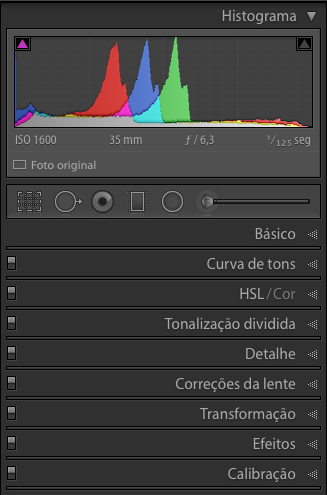
\includegraphics[width=4.3cm]{images/lr_develop_panels.png}};
              \draw[red,ultra thick,rounded corners] (0.15, 4.75) rectangle (4.2, 6.1);
          \end{tikzpicture}
      }
      \column{0.65\textwidth}{
        \begin{itemize}
            \item O Histograma mostra a freqüência do valores percentuais de cada um dos
        canais de cor RGB (vermelho, verde e azul) na imagem.
            \item As \textit{cores} formadas no histograma mostram a combinação dos canais
        naquela freqüência específica.
            \item O histograma nos ajuda a entender os tons que aparecem na foto.
        \end{itemize}
      }
  \end{columns}
\end{frame}

%05
\begin{frame}
  \frametitle{Histograma - Pretos/\textit{Blacks}}
  \begin{columns}
      \column{0.3\textwidth}{
          \begin{tikzpicture}
              \node[anchor=south west,inner sep=0] at (0,0)
                {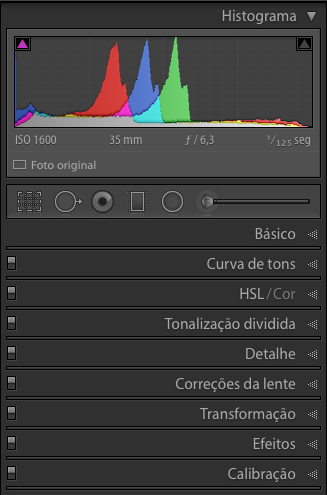
\includegraphics[width=4.3cm]{images/lr_develop_panels.png}};
              \draw[cyan,ultra thick,rounded corners] (0.15, 4.7) rectangle (0.6,6.1);
          \end{tikzpicture}
      }
      \column{0.65\textwidth}{
        \begin{itemize}
            \item Esta região do histograma mostra os tons mais escuros da imagem,
            equivalentes as zonas 0 e 1.
            \item Se triângulo no canto esquerdo superior está colorido,
            um ou mais canais de cor atingiram o valor de 0\%, o preto absoluto.
            \item Posicionar o cursor em cima do triângulo mostra os pontos em 0\%
            na imagem (máscara azul).
        \end{itemize}
      }
  \end{columns}
\end{frame}

%06
\begin{frame}
  \frametitle{\Large Histograma - Sombras/\textit{Shadows}}
  \begin{columns}
      \column{0.3\textwidth}{
          \begin{tikzpicture}
              \node[anchor=south west,inner sep=0] at (0,0)
                {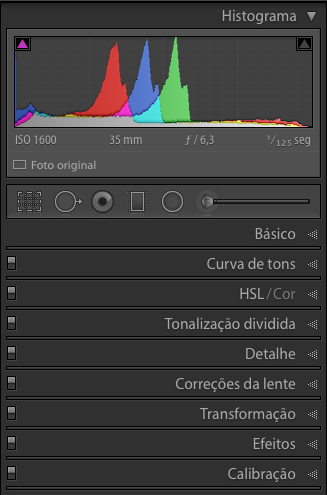
\includegraphics[width=4.3cm]{images/lr_develop_panels.png}};
              \draw[cyan,ultra thick,rounded corners] (0.6, 4.7) rectangle (1.3,6.1);
          \end{tikzpicture}
      }
      \column{0.65\textwidth}{
        \begin{itemize}
            \item Esta região mostra os tons equivalentes as zonas 2 e 3.
        \end{itemize}
      }
  \end{columns}
\end{frame}

%07
\begin{frame}
  \frametitle{Histograma - Tons Médios}
  \begin{columns}
      \column{0.3\textwidth}{
          \begin{tikzpicture}
              \node[anchor=south west,inner sep=0] at (0,0)
                {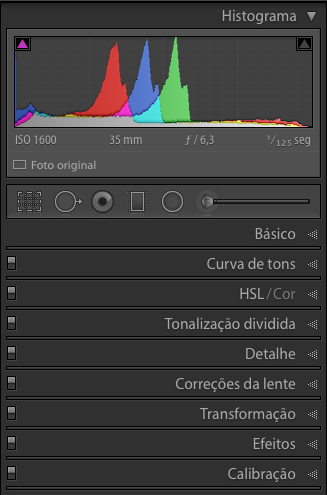
\includegraphics[width=4.3cm]{images/lr_develop_panels.png}};
              \draw[cyan,ultra thick,rounded corners] (1.3, 4.7) rectangle (2.9,6.1);
          \end{tikzpicture}
      }
      \column{0.65\textwidth}{
        \begin{itemize}
            \item Esta região mostra os tons equivalentes as zonas 4, 5 e 6.
            \item Esta região do histograma é a mais afetada pelo controle de \textbf{exposição}.
        \end{itemize}
      }
  \end{columns}
\end{frame}

%08
\begin{frame}
  \frametitle{\Large Histograma - Realces/\textit{Highlights}}
  \begin{columns}
      \column{0.3\textwidth}{
          \begin{tikzpicture}
              \node[anchor=south west,inner sep=0] at (0,0)
                {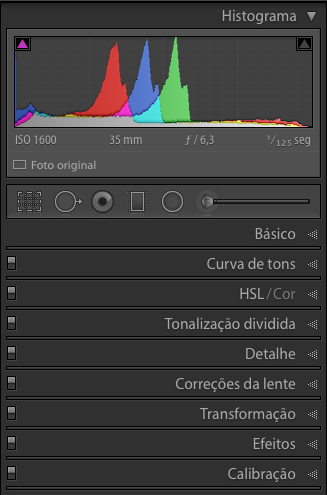
\includegraphics[width=4.3cm]{images/lr_develop_panels.png}};
              \draw[cyan,ultra thick,rounded corners] (2.9, 4.7) rectangle (3.6, 6.1);
          \end{tikzpicture}
      }
      \column{0.65\textwidth}{
      \begin{itemize}
          \item Esta região mostra os tons equivalentes as zonas 7 e 8.
      \end{itemize}
      }
  \end{columns}
\end{frame}

%09
\begin{frame}
  \frametitle{Histograma - Brancos/\textit{Whites}}
  \begin{columns}
      \column{0.3\textwidth}{
          \begin{tikzpicture}
              \node[anchor=south west,inner sep=0] at (0,0)
                {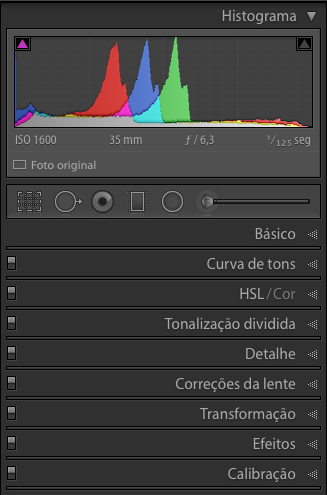
\includegraphics[width=4.3cm]{images/lr_develop_panels.png}};
              \draw[cyan,ultra thick,rounded corners] (3.6, 4.7) rectangle (4.2,6.1);
          \end{tikzpicture}
      }
      \column{0.65\textwidth}{
          \begin{itemize}
              \item Esta região mostra os tons equivalentes as zonas 9 e 10.
              \item Se triângulo no canto esquerdo superior está colorido,
              um ou mais canais de cor atingiram o valor de 100\%, o branco absoluto.
              \item Posicionar o cursor em cima do triângulo mostra os pontos em 100\%
              na imagem (máscara vermelha).
          \end{itemize}
      }
  \end{columns}
\end{frame}

%10
\begin{frame}
  \frametitle{\Large Histograma - Dados de Exposição}
  \begin{columns}
      \column{0.3\textwidth}{
          \begin{tikzpicture}
              \node[anchor=south west,inner sep=0] at (0,0)
                {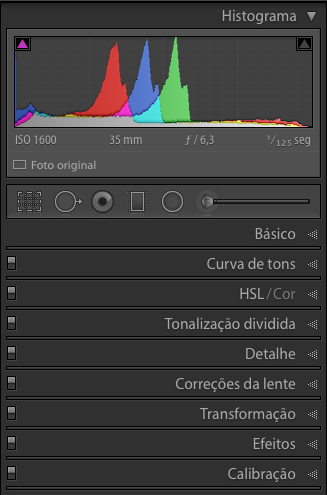
\includegraphics[width=4.3cm]{images/lr_develop_panels.png}};
              \draw[cyan,ultra thick,rounded corners]
                (0.0, 4.43) rectangle (4.3, 4.85);
          \end{tikzpicture}
      }
      \column{0.65\textwidth}{
        \begin{itemize}
            \item Abaixo do histograma são exibidos os dados de exposição da foto.
            \item Se você está com o cursor em cima de uma região da imagem, aparecem
            aqui os percentuais de \textit{vermelho}, \textit{verde} e \textit{azul},
            daquele ponto.
        \end{itemize}
      }
  \end{columns}
\end{frame}

%11
\begin{frame}
  \frametitle{Histograma - Tipo de Arquivo}
  \begin{columns}
      \column{0.3\textwidth}{
          \begin{tikzpicture}
              \node[anchor=south west,inner sep=0] at (0,0)
                {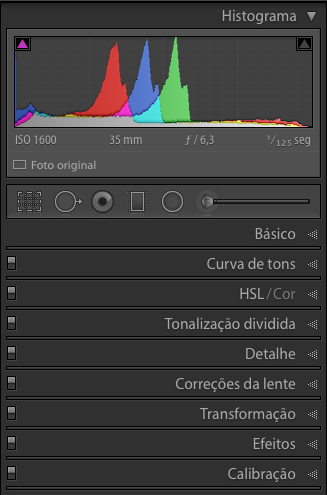
\includegraphics[width=4.3cm]{images/lr_develop_panels.png}};
              \draw[cyan,ultra thick,rounded corners] (0.0, 4.15) rectangle (4.3,4.53);
          \end{tikzpicture}
      }
      \column{0.65\textwidth}{
        \begin{itemize}
            \item Este elemento mostra o tipo de arquivo que está sendo utilizado
            para exibir a imagem.
            \item O arquivo pode ser a foto original, uma visualização inteligente,
            uma combinação do dois, ou uma foto ausente.
            \item No caso de uma foto ausente, a visualização mostrada é a mais simples
            (JPEG) armazenada no banco de dados do Lightroom.
        \end{itemize}
      }
  \end{columns}
\end{frame}

%12
\begin{frame}
    \frametitle{\Large Histograma - Atualização do Processo}
    \begin{columns}
        \column{0.3\textwidth}{
            \begin{tikzpicture}
                \node[anchor=south west,inner sep=0] at (0,0)
                    {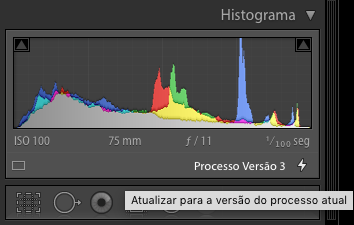
\includegraphics[width=4.3cm]{images/lr_update_process.png}};
                \draw[cyan,ultra thick,rounded corners]
                    (1.5, 0.1) rectangle (4.35,0.9);
            \end{tikzpicture}
        }
        \column{0.65\textwidth}{
            \begin{itemize}
                \item Quando este ícone aparecer em uma imagem, o processo de
                conversão RAW utilizado não é o mais atualizado.
                \item Existem vantagens, principalmente com relação a qualidade
                de imagem, de atualizar o processo de conversão.
                \item Ao atualizar o processo, a forma como a imagem é renderizada
                irá mudar, como cores e tons.
            \end{itemize}
        }
    \end{columns}
\end{frame}

%13
\begin{frame}
    \frametitle{Calibração de Câmera}
    \begin{columns}
        \column{0.3\textwidth}{
            \begin{tikzpicture}
                \node[anchor=south west,inner sep=0] at (0,0)
                    {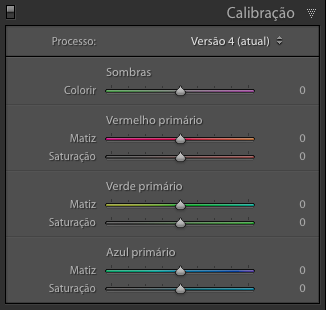
\includegraphics[width=4.3cm]{images/lr_calibration.png}};
                \draw[cyan,ultra thick,rounded corners]
                    (0.4, 3.4) rectangle (4.0,3.8);
                \draw[red,ultra thick,rounded corners]
                    (0.1, 0.1) rectangle (4.2,3.3);
            \end{tikzpicture}
        }
        \column{0.65\textwidth}{
            \begin{itemize}
                \item Permite a seleção do processo (ciano).
                \item Permite alterar a forma como os dados do sensor para as
                cores azul, verde e vermelho são processados (vermelho).
                \item É utilizado para corrigir a resposta de um tipo específico
                de sensor às cores primárias.
                \item É pouco utilizado, e o ideal é que se crie um \textit{preset}
                e não se altere mais a calibração para o mesmo sensor.
            \end{itemize}
        }
    \end{columns}
\end{frame}

%14
\begin{frame}
    \frametitle{\textit{Crop} (Recorte)}
    \begin{columns}
        \column{0.3\textwidth}{
            \begin{tikzpicture}
                \node[anchor=south west,inner sep=0] at (0,0)
                    {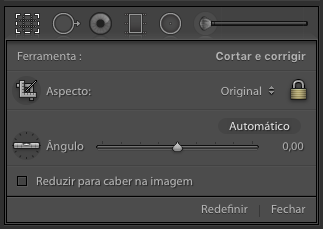
\includegraphics[width=4.3cm]{images/lr_crop.png}};
                \draw[yellow,ultra thick,rounded corners]
                    (0.1, 2.5) rectangle (0.6,3.0);
                \draw[red,ultra thick,rounded corners]
                    (0.1, 0.9) rectangle (4.2,1.4);
                \draw[cyan,ultra thick,rounded corners]
                    (0.1, 1.6) rectangle (4.2,2.05);
            \end{tikzpicture}
        }
        \column{0.65\textwidth}{
            \begin{itemize}
                \item Utilizado para ajustar o corte ou corrigir inclinação na imagem.
                \item Pode utilizar um aspecto específico, escolhido a partir
                de uma lista, ou um formato arbitrário.
                \item É possível corrigir o ângulo de inclinação da foto, ou
                utilizar a ferramenta de nível em uma "linha" que represente uma
                linha horizontal.
            \end{itemize}
        }
    \end{columns}
\end{frame}

%15
\begin{frame}
    \frametitle{Ajustes Básicos}
    \begin{columns}
        \column{0.3\textwidth}{
            \begin{tikzpicture}
                \node[anchor=south west,inner sep=0] at (0,0)
                    {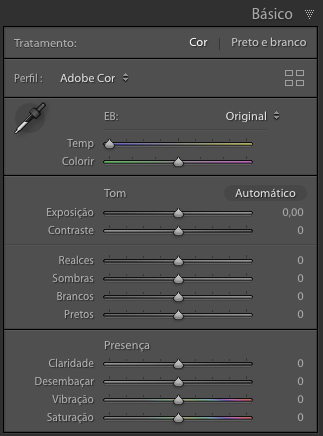
\includegraphics[width=4.3cm]{images/lr_basic.png}};
                \draw[cyan,ultra thick,rounded corners]
                    (2.4, 5.1) rectangle (4.2, 5.4);
            \end{tikzpicture}
        }
        \column{0.65\textwidth}{
            \begin{itemize}
                \item Os ajustes da imagem começam por este painel.
                \item A interface do Lightroom é pensada para que os ajustes sejam
                feitos na ordem que aparecem na interface.
                \item Nesse painel são feitos os ajustes globais de tons e cores.
                \item Em destaque, a opção de escolha de tratamento em cor ou P\&B.
            \end{itemize}
        }
    \end{columns}
\end{frame}

%16
\begin{frame}
    \frametitle{Ajustes Básicos - Perfil}
    \begin{columns}
        \column{0.3\textwidth}{
            \begin{tikzpicture}
                \node[anchor=south west,inner sep=0] at (0,0)
                    {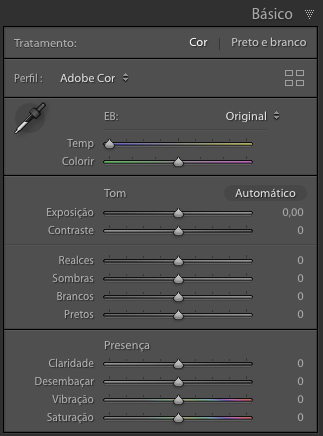
\includegraphics[width=4.3cm]{images/lr_basic.png}};
                \draw[cyan,ultra thick,rounded corners]
                    (0.1, 4.6) rectangle (4.2,5.0);
            \end{tikzpicture}
        }
        \column{0.65\textwidth}{
            \begin{itemize}
                \item Os perfis indicam ao conversor RAW do Lightroom como tratar
                as cores, de acordo com o estilo escolhido.
                \item Podemos escolher um tipo de perfil e associá-lo a uma câmera,
                e este perfil será o perfil padrão para essa câmera específica.
                \item Os perfis apresentados na lista de perfis são os "favoritos",
                escolhidos na aba de pefis, acessível através do botão à esquerda.
            \end{itemize}
        }
    \end{columns}
\end{frame}

%17
\begin{frame}
    \frametitle{Navegador de Pefis - Lista}
    \begin{columns}
        \column{0.3\textwidth}{
            \begin{tikzpicture}
                \node[anchor=south west,inner sep=0] at (0,0)
                    {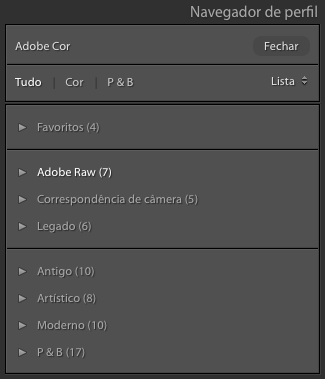
\includegraphics[width=4.3cm]{images/lr_profile.png}};
                \draw[cyan,ultra thick,rounded corners]
                    (0.1, 2.2) rectangle (4.2,2.6);
                \draw[red,ultra thick,rounded corners]
                    (0.1, 0.1) rectangle (4.2,1.7);
            \end{tikzpicture}
        }
        \column{0.65\textwidth}{
            \begin{itemize}
                \item O Lightroom traz vários perfis prontos para uso.
                \item Alguns perfis são baseados na experiência da Adobe. (Thomas Knoll).
                \item Outros perfis tentam imitar as configurações das câmeras (ciano).
                \item Existem também perfis que criam ajustes "artísticos" para a imagem (vermelho).
            \end{itemize}
        }
    \end{columns}
\end{frame}

%18
\begin{frame}
    \frametitle{Navegador de Pefis - Grade}
    \begin{columns}
        \column{0.3\textwidth}{
            \begin{tikzpicture}
                \node[anchor=south west,inner sep=0] at (0,0)
                    {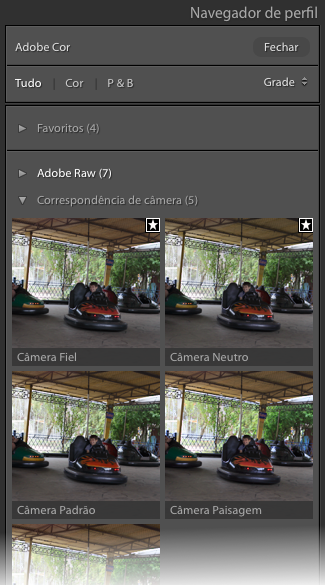
\includegraphics[width=3.5cm]{images/lr_profile_grid.png}};
                \draw[cyan,ultra thick,rounded corners]
                    (3.15, 3.70) rectangle (3.5, 4.05);
            \end{tikzpicture}
        }
        \column{0.65\textwidth}{
            \begin{itemize}
                \item Usando o modo \textbf{grade}, é possível tem uma previsão
                do efeito gerado ao aplicar o perfil.
                \item A estrela (destaque) pode ser habilitada, fazendo com que
                o perfil apareça na lista do painel \textbf{básico}.
            \end{itemize}
        }
    \end{columns}
\end{frame}

%19
\begin{frame}
    \frametitle{Navegador de Pefis - Grande}
    \begin{columns}
        \column{0.3\textwidth}{
            \begin{tikzpicture}
                \node[anchor=south west,inner sep=0] at (0,0)
                    {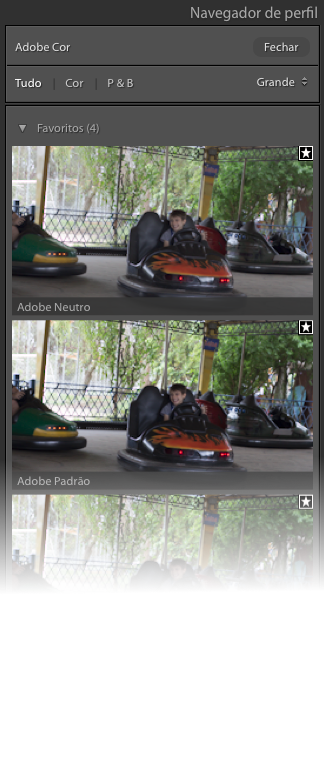
\includegraphics[width=3.5cm]{images/lr_profile_big.png}};
            \end{tikzpicture}
        }
        \column{0.65\textwidth}{
            \begin{itemize}
                \item O modo \textbf{Grande} do navegador de perfis auxilia a
                ver com mais detalhes os efeitos de cada perfil.
            \end{itemize}
        }
    \end{columns}
\end{frame}

%20
\begin{frame}
    \frametitle{\Large Ajustes Básicos - Balanço de Branco}
    \begin{columns}
        \column{0.3\textwidth}{
            \begin{tikzpicture}
                \node[anchor=south west,inner sep=0] at (0,0)
                    {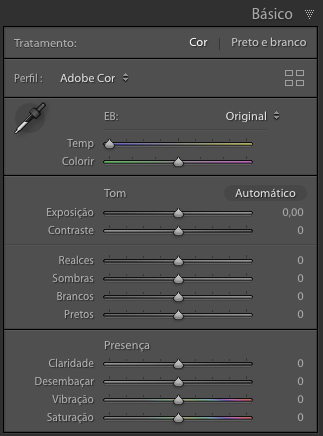
\includegraphics[width=4.3cm]{images/lr_basic.png}};
                \draw[cyan,ultra thick,rounded corners]
                    (0.1, 3.45) rectangle (4.15,4.55);
            \end{tikzpicture}
        }
        \column{0.65\textwidth}{
            \begin{itemize}
                \item Neste painel pode-se corrigir desvios de temperatura de cor,
                ou \textit{tint}.
                \item É possivel utilizar perfis, ou utilizar o ajuste automático.
                \item Com o \textit{conta-gotas}, seleciona-se um ponto da imagem
                com um tom que deveria ser \textit{neutro}, e ajustar o balanço
                de branco para corrigir este ponto.
            \end{itemize}
        }
    \end{columns}
\end{frame}

%21
\begin{frame}
    \frametitle{\Large Ajustes Básicos - Exposição Básica}
    \begin{columns}
        \column{0.3\textwidth}{
            \begin{tikzpicture}
                \node[anchor=south west,inner sep=0] at (0,0)
                    {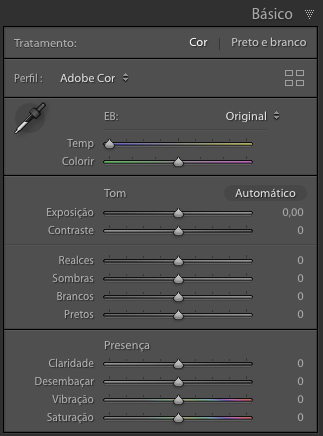
\includegraphics[width=4.3cm]{images/lr_basic.png}};
                \draw[cyan,ultra thick,rounded corners]
                    (0.1, 2.57) rectangle (4.25,3.38);
            \end{tikzpicture}
        }
        \column{0.65\textwidth}{
            \begin{itemize}
                \item O \textit{slider} \textbf{Exposição} ajusta a exposição geral
                da imagem em \textit{stops}.
                \item A exposição afeta, principalmente, os tons médios.
                \item O \textbf{contraste}, afeta o contraste global da imagem,
                influenciando, também, a saturação de cores.
            \end{itemize}
        }
    \end{columns}
\end{frame}

%22
\begin{frame}
    \frametitle{Ajustes Básicos - Tons}
    \begin{columns}
        \column{0.3\textwidth}{
            \begin{tikzpicture}
                \node[anchor=south west,inner sep=0] at (0,0)
                    {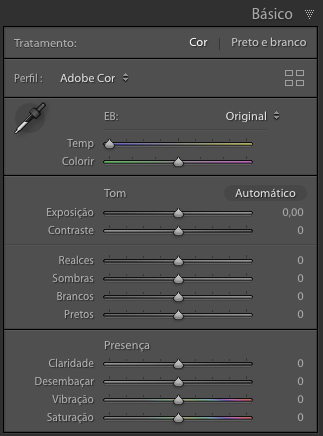
\includegraphics[width=4.3cm]{images/lr_basic.png}};
                \draw[cyan,ultra thick,rounded corners]
                    (0.1, 1.45) rectangle (4.25,2.58);
            \end{tikzpicture}
        }
        \column{0.65\textwidth}{
            \begin{itemize}
                \item O \textit{slider} \textbf{Realces}, ajusta os tons das zonas 7 e 8.
                \item O \textit{slider} \textbf{Sombras}, ajusta os tons das zonas 2 e 3.
                \item O \textit{slider} \textbf{Brancos}, ajusta o valor máximo dos brancos.
                \item O \textit{slider} \textbf{Pretos}, ajusta o valor mínimo dos pretos.
            \end{itemize}
        }
    \end{columns}
\end{frame}

%23
\begin{frame}
    \frametitle{Ajustes Básicos - Presença}
    \begin{columns}
        \column{0.3\textwidth}{
            \begin{tikzpicture}
                \node[anchor=south west,inner sep=0] at (0,0)
                    {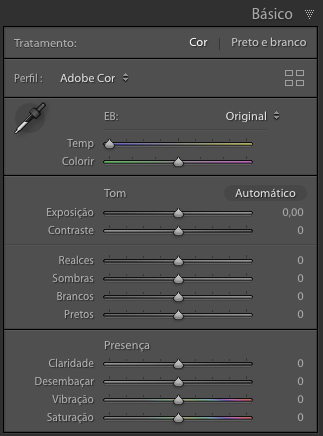
\includegraphics[width=4.3cm]{images/lr_basic.png}};
                \draw[cyan,ultra thick,rounded corners]
                    (0.1, 0.05) rectangle (4.25, 1.35);
            \end{tikzpicture}
        }
        \column{0.65\textwidth}{
            \begin{itemize}
                \item O \textit{slider} \textbf{Claridade}, altera o contraste entre os tons médios.
                \item O \textit{slider} \textbf{Desembaçar}, modifica o contraste de forma a diminuir
                o efeito \textit{haze}.
                \item O \textit{slider} \textbf{Vibração}, é um ajuste de saturação que evita a super-saturação.
                \item O \textit{slider} \textbf{Saturação}, ajusta a saturação de todas as cores.
            \end{itemize}
        }
    \end{columns}
\end{frame}

%24
\begin{frame}
    \frametitle{Curva de Tons - Paramétrica}
    \begin{columns}
        \column{0.3\textwidth}{
            \begin{tikzpicture}
                \node[anchor=south west,inner sep=0] at (0,0)
                    {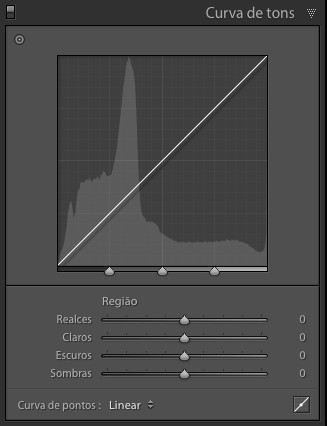
\includegraphics[width=4.3cm]{images/lr_tone_curve_parametric.png}};
            \end{tikzpicture}
        }
        \column{0.65\textwidth}{
            \begin{itemize}
                \item Este painel permite ajustar a curva de resposta dos canais
                da imagem.
                \item É possível modificar os canais RGB de forma conjunta ou independente.
                \item Na forma \textit{paramétrica}, o Lightroom adiciona limites à curva.
            \end{itemize}
        }
    \end{columns}
\end{frame}

%25
\begin{frame}
    \frametitle{Curva de Tons - Livre}
    \begin{columns}
        \column{0.3\textwidth}{
            \begin{tikzpicture}
                \node[anchor=south west,inner sep=0] at (0,0)
                    {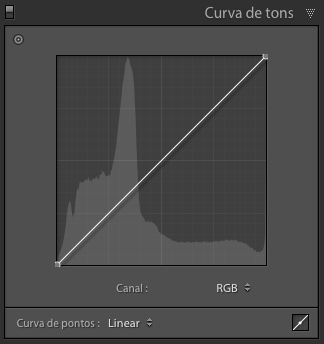
\includegraphics[width=4.3cm]{images/lr_tone_curve.png}};
                \draw[cyan,ultra thick,rounded corners]
                    (3.80, 0.05) rectangle (4.25,0.5);
            \end{tikzpicture}
        }
        \column{0.65\textwidth}{
            \begin{itemize}
                \item No ajuste \textit{livre} da curva de tons, nenhum limite no ajuste da curva é imposto.
                \item A troca de modo é realizada pelo botão em destaque.
            \end{itemize}
        }
    \end{columns}
\end{frame}

%26
\begin{frame}
    \frametitle{Ajuste de Cores - HSL}
    \begin{columns}
        \column{0.3\textwidth}{
            \begin{tikzpicture}
                \node[anchor=south west,inner sep=0] at (0,0)
                    {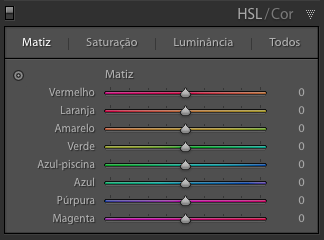
\includegraphics[width=4.3cm]{images/lr_hsl.png}};
            \end{tikzpicture}
        }
        \column{0.65\textwidth}{
            \begin{itemize}
                \item Permite o ajuste indiviual de canais de cores, utilizando
                uma interface com o modo Matiz (\textit{Hue}), Saturação (\textit{Saturation}),
                e Luminosidade (\textit{Lightness}).
            \end{itemize}
        }
    \end{columns}
\end{frame}

%27
\begin{frame}
    \frametitle{Ajuste de Cores - Color}
    \begin{columns}
        \column{0.3\textwidth}{
            \begin{tikzpicture}
                \node[anchor=south west,inner sep=0] at (0,0)
                    {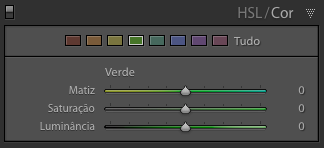
\includegraphics[width=4.3cm]{images/lr_color.png}};
            \end{tikzpicture}
        }
        \column{0.65\textwidth}{
            \begin{itemize}
                \item Permite o ajuste indiviual de canais de cores, utilizando
                uma interface que mostra as cores, e mostra, para a cor selecionada,
                os valores de Matiz, Saturação e Luminosidade.
            \end{itemize}
        }
    \end{columns}
\end{frame}

%28
\begin{frame}
    \frametitle{Ajuste de Cores - P\&B}
    \begin{columns}
        \column{0.3\textwidth}{
            \begin{tikzpicture}
                \node[anchor=south west,inner sep=0] at (0,0)
                    {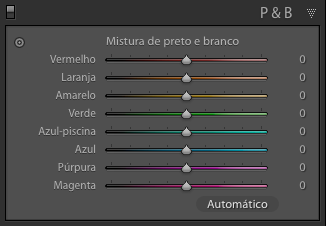
\includegraphics[width=4.3cm]{images/lr_black_white.png}};
            \end{tikzpicture}
        }
        \column{0.65\textwidth}{
            \begin{itemize}
                \item Substitui o painel de ajuste de cores quando o modo da imagem é
                alterado para \textbf{Preto e Branco}.
                \item Ajusta a resposta de tons a uma determinada cor.
                \item É utilizado para simular o efeito de filtros analógicos.
            \end{itemize}
        }
    \end{columns}
\end{frame}

%29
\begin{frame}
    \frametitle{Tonalização Dividida}
    \begin{columns}
        \column{0.3\textwidth}{
            \begin{tikzpicture}
                \node[anchor=south west,inner sep=0] at (0,0)
                    {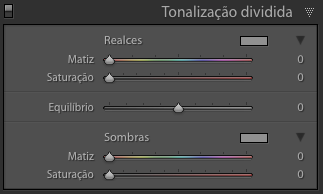
\includegraphics[width=4.3cm]{images/lr_split_toning.png}};
            \end{tikzpicture}
        }
        \column{0.65\textwidth}{
            \begin{itemize}
                \item Permite adicionar duas cores para tonalizar áreas de sombra e luzes.
                \item Pode ser utirizado tanto em imagens coloridas como P\&B.
                \item Em P\&b tem um efeito semelhante ao \textit{duotone}.
            \end{itemize}
        }
    \end{columns}
\end{frame}

%30
\begin{frame}
    \frametitle{Detalhes}
    \begin{columns}
        \column{0.3\textwidth}{
            \begin{tikzpicture}
                \node[anchor=south west,inner sep=0] at (0,0)
                    {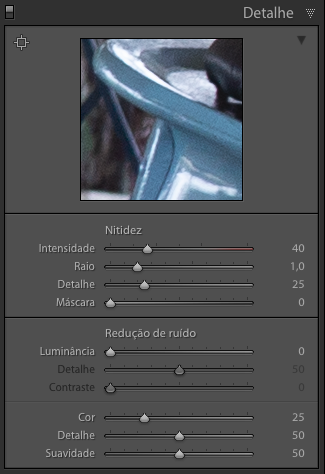
\includegraphics[width=4.3cm]{images/lr_sharpening.png}};
            \draw[cyan,ultra thick,rounded corners]
                (0.1, 2.15) rectangle (4.2,3.4);
            \draw[red,ultra thick,rounded corners]
                (0.1, 0.1) rectangle (4.2,2.10);
            \end{tikzpicture}
        }
        \column{0.65\textwidth}{
            \begin{itemize}
                \item Ajustes de Nitidez (ciano) e Redução de Ruído (vermelho).
                \item Use, sempre, em 100\% (1:1) ou 200\% (2:1).
                \item Em monitores comuns, com 98 a 120 dpi, utilize 50\% (1:2)
                para simular como ficaria a impressão.
            \end{itemize}
        }
    \end{columns}
\end{frame}

%31
\begin{frame}
    \frametitle{Nitidez - Intensidade e Raio}
    \begin{columns}
        \column{0.3\textwidth}{
            \begin{tikzpicture}
                \node[anchor=south west,inner sep=0] at (0,0)
                    {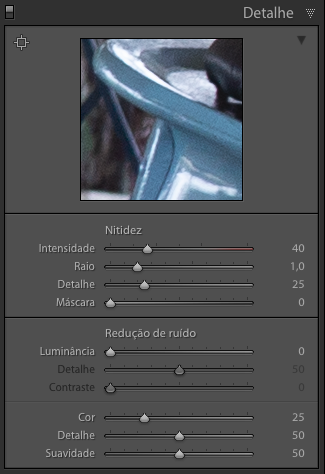
\includegraphics[width=4.3cm]{images/lr_sharpening.png}};
            \draw[cyan,ultra thick,rounded corners]
                (0.1, 2.55) rectangle (4.2,3.2);
            \end{tikzpicture}
        }
        \column{0.65\textwidth}{
            \begin{itemize}
                \item A nitidez é realizada de forma semelhante ao Unsharp Mask.
                \item A \textbf{intensidade} regula o quanto o efeito é aplicado.
                \item O \textbf{raio} regula o quão "longe" a análise é realizada.
            \end{itemize}
        }
    \end{columns}
\end{frame}

%32
\begin{frame}
    \frametitle{Nitidez - Detalhes e Máscara}
    \begin{columns}
        \column{0.3\textwidth}{
            \begin{tikzpicture}
                \node[anchor=south west,inner sep=0] at (0,0)
                    {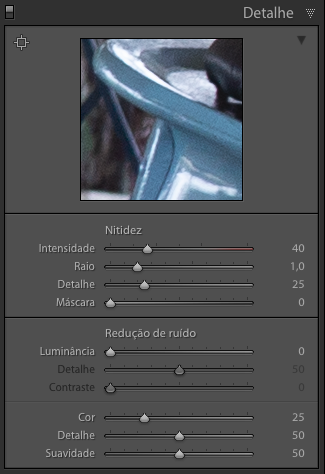
\includegraphics[width=4.3cm]{images/lr_sharpening.png}};
            \draw[cyan,ultra thick,rounded corners]
                (0.1, 2.05) rectangle (4.2,2.8);
            \end{tikzpicture}
        }
        \column{0.65\textwidth}{
            \begin{itemize}
                \item Os \textbf{detalhes}, buscam aumentar o contraste local em
                elementos com poucos pixels (pode aumentar a visibilidade de ruído).
                \item A \textbf{máscara}, cria um filtro definindo quão próximo ou
                longe das bordas dos objetos a nitidez será aplicada.
            \end{itemize}
        }
    \end{columns}
\end{frame}

%33
\begin{frame}
    \frametitle{Detalhes - Redução de Ruído}
    \begin{columns}
        \column{0.3\textwidth}{
            \begin{tikzpicture}
                \node[anchor=south west,inner sep=0] at (0,0)
                    {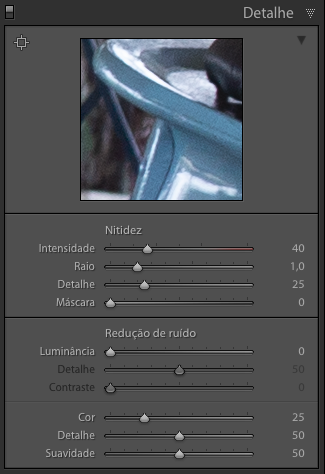
\includegraphics[width=4.3cm]{images/lr_sharpening.png}};
            \draw[cyan,ultra thick,rounded corners]
                (0.1, 1.00) rectangle (4.2,2.0);
            \draw[red,ultra thick,rounded corners]
                (0.1, 0.1) rectangle (4.2,0.95);
            \end{tikzpicture}
        }
        \column{0.65\textwidth}{
            \begin{itemize}
                \item Aplica algoritmos de redução de ruído luminoso (ciano) ou
                de cor (vermelho).
                \item O primeiro item define a quantidade de redução de ruído a
                ser aplicada.
                \item Os \textit{sliders} \textbf{detalhe} e \textbf{contraste}
                buscam recuperar um pouco os detalhes e contraste perdidos pela
                redução de ruído.
            \end{itemize}
        }
    \end{columns}
\end{frame}

%34
\begin{frame}
    \frametitle{Correção de Lentes}
    \begin{columns}
        \column{0.3\textwidth}{
            \begin{tikzpicture}
                \node[anchor=south west,inner sep=0] at (0,0)
                    {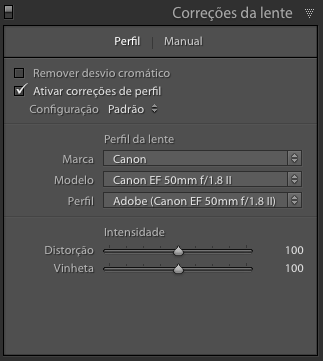
\includegraphics[width=4.3cm]{images/lr_lens_correction.png}};
            \end{tikzpicture}
        }
        \column{0.65\textwidth}{
            \begin{itemize}
                \item A correção de lentes automática, aplica um perfil de lente
                à imagem.
                \item É possível controlar a intensidade do ajuste de distorção
                e da vinheta.
                \item Neste painel você também pode corrigir a desvio cromático.
                \item As duas configurações são indicadas para serem utilizadas sempre.
            \end{itemize}
        }
    \end{columns}
\end{frame}

%35
\begin{frame}
    \frametitle{Correção de Lentes Manual}
    \begin{columns}
        \column{0.3\textwidth}{
            \begin{tikzpicture}
                \node[anchor=south west,inner sep=0] at (0,0)
                    {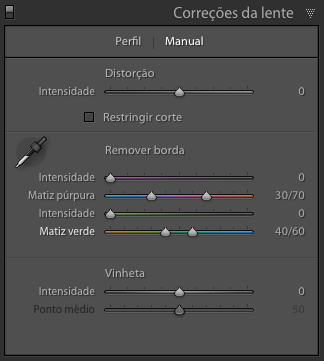
\includegraphics[width=4.3cm]{images/lr_lens_correction_manual.png}};
            \end{tikzpicture}
        }
        \column{0.65\textwidth}{
            \begin{itemize}
                \item No ajuste de lentes manual, é possível corrigir a distorção
                da lente para dentro (\textit{pincushion}) ou para fora (\textit{barrel}).
                \item É possível corrigir, com bastante precisão, o desvio cromático.
                \item Há também mais controle sobre a correção de vinheta.
                \item É possível mesclar as distorções automáticas e manual.
            \end{itemize}
        }
    \end{columns}
\end{frame}

%36
\begin{frame}
    \frametitle{Transformação (\textit{Upright})}
    \begin{columns}
        \column{0.3\textwidth}{
            \begin{tikzpicture}
                \node[anchor=south west,inner sep=0] at (0,0)
                    {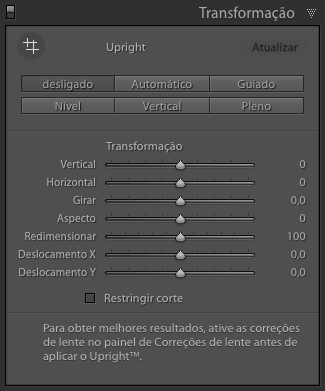
\includegraphics[width=4.3cm]{images/lr_upright.png}};
            \end{tikzpicture}
        }
        \column{0.65\textwidth}{
            \begin{itemize}
                \item Correção da geometria da foto, causada pela perspectiva e
                transformação 3D$\rightarrow$2D.
                \item É melhor habilitar a correção de lentes \textit{antes} de
                utilizar essa correção (ou atualizar a correção automática após
                habilitar a correção de lentes).
                \item O modo \textbf{Guiado} permite que até 4 linhas sejam utilizadas
                como guias.
            \end{itemize}
        }
    \end{columns}
\end{frame}

%37
\begin{frame}
    \frametitle{Efeitos}
    \begin{columns}
        \column{0.3\textwidth}{
            \begin{tikzpicture}
                \node[anchor=south west,inner sep=0] at (0,0)
                    {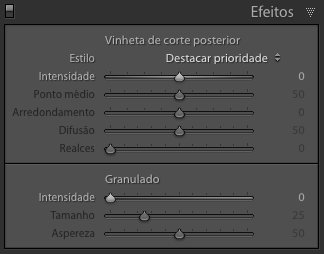
\includegraphics[width=4.3cm]{images/lr_effects.png}};
            \end{tikzpicture}
        }
        \column{0.65\textwidth}{
            \begin{itemize}
                \item Aplica uma vinheta na imagem final, ou adiciona "ruído" que
                tenta imitar o \textit{grão} de filmes fotográficos.
                \item A vinheta pode ser mais escura ou mais clara que a imagem.
                \item O grão pode ser utilizado para melhorar a nitidez, principalmente
                em fotos que precisaram de uma grande quantidade de redução de ruído.
            \end{itemize}
        }
    \end{columns}
\end{frame}

%
% Up in the file...
% Local Adjustment
%
% History
% left_buttons
% right_buttons
% presets
% Snapshots
%
% Toolbar (reference_view_launch, Spot healing)
%
% Copy/Preset selection screen
%30
\begin{frame}
    \frametitle{}
    \begin{columns}
        \column{0.3\textwidth}{
            \begin{tikzpicture}
                \node[anchor=south west,inner sep=0] at (0,0)
                    {
\includegraphics[width=4.3cm]{images/lr_right_buttons.png}};
                \draw[cyan,ultra thick,rounded corners]
                    (0.1, 4.5) rectangle (3.5,5.0);
            \end{tikzpicture}
        }
        \column{0.65\textwidth}{
            \begin{itemize}
                \item None
            \end{itemize}
        }
    \end{columns}
\end{frame}

%xx
\finalframe[Vamos gastar o obturador!]{rafasgj@gmail.com}

%xx+1
\begin{frame}
    \frametitle{Bibliografia}
    \begin{itemize}[]
      \item Adobe Lightroom Classic CC Learn \& Support\\
      \textbf{\small \url{https://helpx.adobe.com/support/lightroom.html}}

      \item \textbf{Luminous-Landscape} \begin{itemize}
          \item Adobe Lightroom CC/6 Tutorial Videos\\
              {\footnotesize \url{https://luminous-landscape.com/videos/adobe-lightroomcc6-2015/}}
          \item Camera to Print \& Screen\\
              {\footnotesize \url{https://luminous-landscape.com/videos/camera-print-screen/}}
          \item Guide to Capture One Pro 10\\
              {\footnotesize \url{https://luminous-landscape.com/videos/guide-capture-one-10/}}
      \end{itemize}
    \end{itemize}
\end{frame}

\end{document}
